\section{KitchenDesigner}

We want to build an application, KitchenDesigner, that allows users to define the layout of kitchens and to insert in such layouts the furniture and appliances (refrigerators, stoves, dishwashers, etc.) that go in them.
For simplicity, we consider only rooms that have rectangular shape. 
Users can define the physical features of the room (length, width, height). 
Moreover, they can add pieces of furniture and appliances, and move them around. 
The position of each piece of furniture/appliance is given by the 3D coordinates of the lower left corner of the bottom side of the item, and by its orientation (which is the angle with respect to the $x$ axis, and which can only be a multiple of 90 degrees).
Users register with the application to be able to store and retrieve their designs. 
After a user finalizes his/her kitchen design, he/she can ask to have the kitchen delivered to a desired address; in this case, the kitchen is sent to production, and the user is given a probable date of delivery (producing a kitchen can take a few days, or even weeks). 
For simplicity, we do not consider payment. 
When the kitchen is ready to be delivered, the user is notified of the confirmed date of delivery.
The system keeps track of the designs created by users, to identify the most common combinations of pieces of furniture and appliances. 
Hence, upon request by a user, given a draft layout for the kitchen, the system returns a list of possible pieces of furniture and appliances that might be added to that kitchen.
Assuming you need to implement system KitchenDesigner analyzed above, identify the most relevant components and interfaces describing them through UML Component or Class Diagrams.
Provide a brief description of each component. 
For each interface identified in the previous point, list the operations that it provides. 
You do not need to precisely specify operation parameters; however, you should give each operation a meaningful enough name to understand what it does; you can also briefly describe what information operations use/produce.
Define a runtime-level Sequence Diagram describing the interaction that occurs among the KitchenDesigner components when the user asks for a list of suggested elements to be added to the kitchen. 
If useful, provide a brief description of the defined Sequence Diagram.

\paragraph*{Solution}
The requested UML Component diagram is as follows: 
\begin{figure}[H]
    \centering
    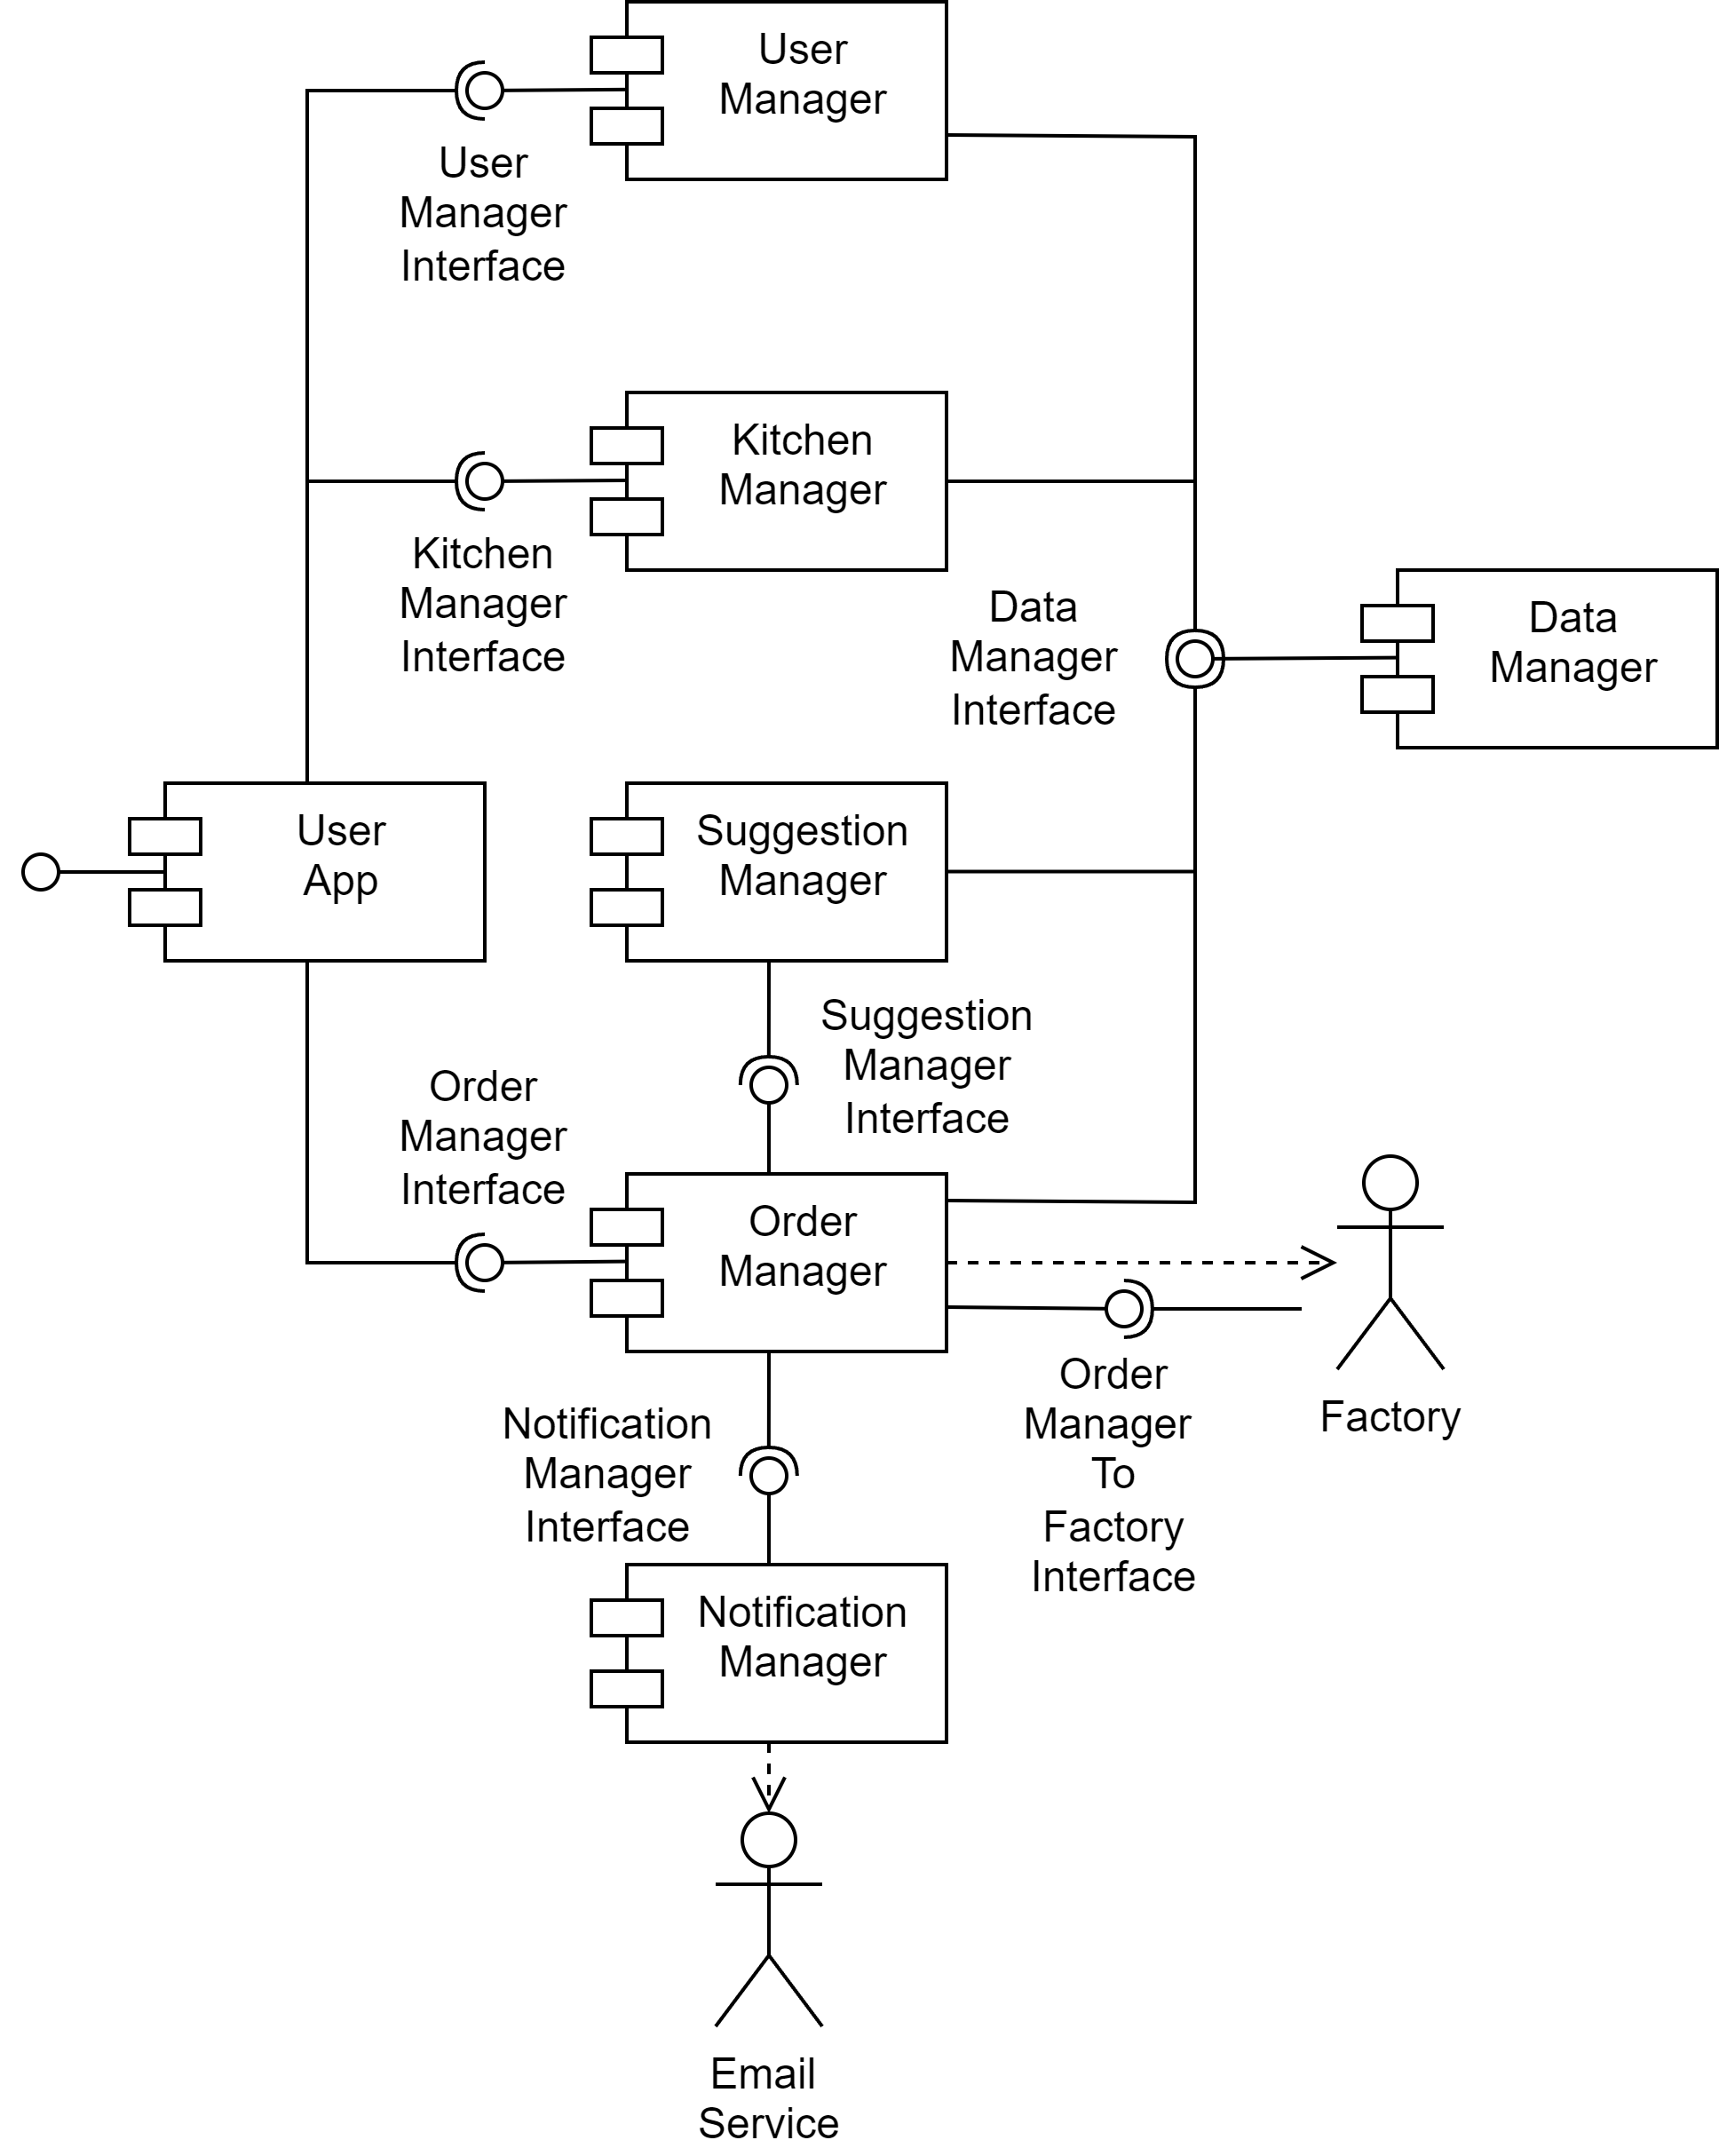
\includegraphics[width=0.4\linewidth]{images/cd.png}
\end{figure}

The component \texttt{UserApp} is the front-end for users. 
It allows them to interact with the system by offering the following functions through interface \textit{UserAppI}:
\begin{itemize}
    \item Register, which has as input the user data. 
    \item Login, which has as inputs the userId and the password.
    \item Create a new kitchen project, which has as input the name. 
    \item Set the dimensions of the kitchen, which has as input the dimensions.
    \item Add an item to kitchen, which has as input the item to be added.
    \item Move item in kitchen, which has as input the item to be moved and the new position.
    \item Remove item from kitchen, which has as input the item to be removed.
    \item Ask for a suggestion, which returns the suggested elements.
    \item Finalize kitchen.
    \item Place order.
\end{itemize}
The module can keep track of the current kitchen being designed, so the user operates on the open project, and the information does not need to be included in the calls each time.

The component \texttt{UserManager} offers, through interface \texttt{UserManagerI}, the basic functions for handling users:
\begin{itemize}
    \item Register, which has as input the user info. 
    \item Login, which has as inputs the userId and password. 
\end{itemize}

The component \texttt{KitchenManager} provides the interface \texttt{KitchenManagerI}, which handles functions related to the management of kitchens (excluding placing the order, which is handled by another component):
\begin{itemize}
    \item Create a new kitchen project, which has as input the name. 
    \item Set the dimensions of the kitchen, which has as inputs the kitchenId and the dimensions. 
    \item Add an item to kitchen, which has as inputs the kitchenId and the item to be added. 
    \item Move item in kitchen, which has as input the kitchenId, the item to be moved and the new position. 
    \item Remove item from kitchen, which has as inputs the kitchenId and the item to be removed. 
    \item Ask for a suggestion, which has as input the kitchenId and returns the suggested elements. 
    \item Finalize kitchen, which has as input the kitchenId. 
\end{itemize}
These operations are similar to those offered by the UserApp, but they also include the Id of the kitchen which should be modified.

The component \texttt{SuggestionManager} provides, through interface \texttt{SuggestionsManagerI}, functions related to the retrieval of suggestions:
\begin{itemize}
    \item Get suggestion, which has as input the kitchenId.
\end{itemize}
The idea is that the component periodically retrieves kitchen designs from the \texttt{DataManager}, mines them, and identifies which combinations of items are most common. 
Hence, it only provides a single function, for getting the outcome of this mining. 
Hence, the computation is mostly offline, the get suggestion function compares what is present in the kitchen with what is most common, and suggests additional elements.



The component \texttt{OrderManager} provides, through interfaces \texttt{OrderManagerI} and \texttt{OrderManager2FactoryI} functions related to the management of orders. 
These are used by two different clients. 
The interface \texttt{OrderManagerI} is used by \texttt{UserApp} and provides the following function: 
\begin{itemize}
\item Place order, which has as input the kitchenId.
    It is used to start the process to produce a kitchen. 
    To handle the order the OrderManager needs to notify the factory of the new order. 
    The handling of the order, and in particular its creation, is outside the scope of the \texttt{KitchenDesigner} application; this is represented in the diagram by the fact that there is an interaction with the factory. 
    When the order is complete, the \texttt{OrderManager} is informed of this through interface \texttt{OrderManager2FactoryI} (to be used by the external actor factory) which provides the following operation:
    \begin{itemize}
        \item Kitchen completed, which has as input the kitchenId. 
            Which simply informs the OrderManager that the kitchen is indeed ready (hence the user can be notified of the date of its actual delivery).
    \end{itemize}
\end{itemize}

The component \texttt{NotificationManager} handles the notification to users, in particular updates on when the kitchen will be delivered. 
It provides the following function through interface \texttt{NotificationManagerI}:
\begin{itemize}
    \item Notify user, which has as inputs the message to be sent and the recipient. 
        The notification is sent as an email, and for this reason it goes through an email server, which is an external component, outside the system.
\end{itemize}

The component \texttt{DataManager} handles the data of the system, which consists essentially of users and kitchens. 
It provides interface \texttt{DataManagerI}, which includes all necessary functions to handle CRUD operations on data.
The only backend component that does not need to interact with \texttt{DataManager} is \texttt{NotificationManager}, because it relies on information provided by \texttt{OrderManager}.

The requested UML Sequence diagram is depicted below: 
\begin{figure}[H]
    \centering
    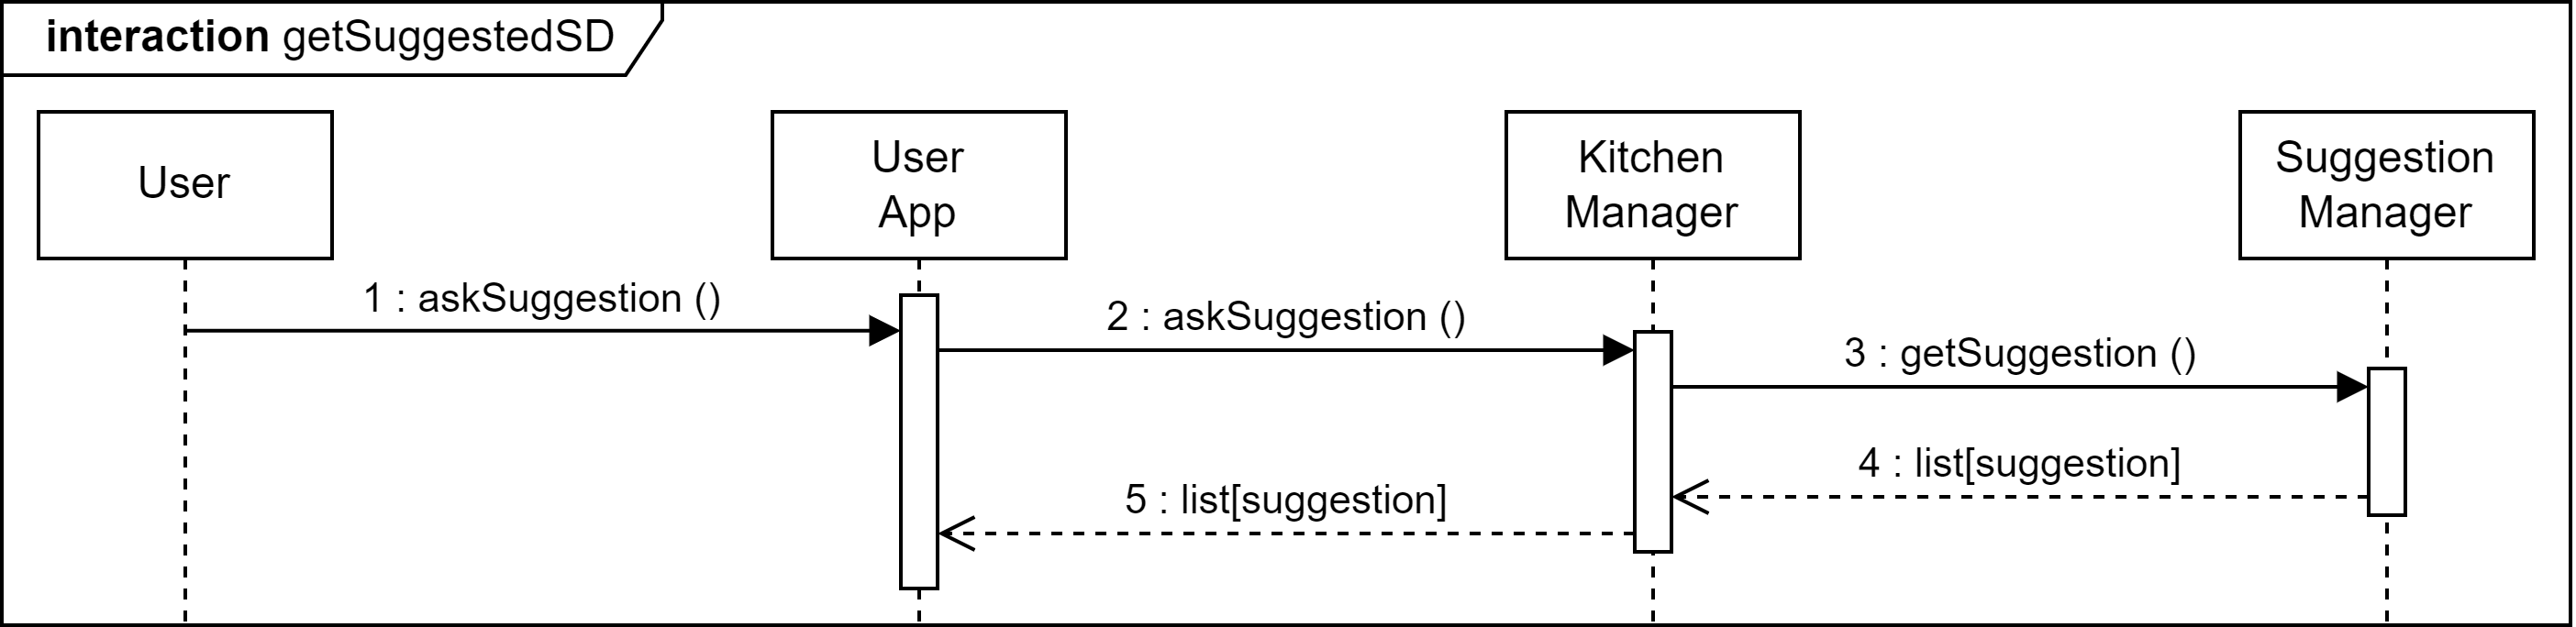
\includegraphics[width=0.9\linewidth]{images/sd2.png}
\end{figure}
Mining of the designs is done asynchronously, not when a suggestion is requested, but offline, so it is not represented in this interaction.